\chapter{Theoretische Grundlagen}
\label{ch:Theoretische Grundlagen}
Dieses Kapitel dient als Einführung in die Grundlagen von Filtern, sowie die Themenkomplexe Künstliche Intelligenz und \ac*{iot}. Hierbei wird ein kurzer Überblick über die genannten Themenbereiche geliefert, sowie für die vorliegende Arbeit relevante Unterthemen näher erläutert.
\section{Grundlagen Filter}
Filter als Bau- und Maschinenelement zur Filtration von flüssigen und gasförmigen Medien existieren in einer Vielzahl von Bauweisen und Wirkmechanismen 
(s. \ref{fi:klassifikation_filtration} und \ref{sec:filtereffekte}). Im Rahmen dieser Arbeit soll nicht auf Flüssigkeitsfilter und auch nicht auf Gasabsorptionsfilter eingegangen werden. Der Fokus wird auf abscheidende Filter, welche in industriellen Szenarien z.B. zur Abscheidung von Arbeitsstäuben und Verunreinigungen der Außenluft (\ac{oda}) eingesetzt werden, gelegt. \newline Der Wirkmechanismus ist hierbei grundsätzlich folgender: Eine Seite des Filters wird mit sog. Rohgas angeströmt, das Filtermedium scheidet hierbei über diverse Filtereffekte die Verunreinigungen ab, so dass auf der Reingasseite ein Gasgemisch austritt, welches weniger Verunreinigungen enthält. Dies erfolgt im Fall von Luftfiltern in der Regel durch faserbasierte Filtermedien, welche insbesondere bei Applikationen eingesetzt werden, bei denen es auf eine besonders wirksame Abscheidung ankommt.\cite{Staubabscheidung} Diese Faserfilter lassen sich, je nach Anwendungsbereich und dem hieraus resultierenden Aufbau, sowie Betriebsweise in zwei Gruppen aufteilen: Speicherfilter (bzw. Tiefenfilter) und Abreinigungsfilter (bzw. Oberflächenfilter, Kuchenfilter). \cite{AbscheidungPartikel} \newline
Die in dieser Arbeit behandelten Filter lassen sich also nach Kraume \ref{fi:klassifikation_filtration} wie folgt zuordnen: Die treibende Kraft bei den untersuchten Filtern ist der Druck, die Prozessführung ist die Tiefenfiltration. Streng genommen würde ein Wechsel der Filtermedien einen diskontinuierlichen Prozess bedingen, allerdings meint eine diskontinuierliche Betriebsweise in diesem Kontext z.B. die periodischen Abreinigungsphasen bei Oberflächenfiltern (s. \ref{sec:filterbauarten}), weswegen die für diese Arbeit relevanten Luftfilter einem kontinuierlichen Prozess zuzuordnen sind. 
\begin{figure}[H]
    \begin{center}
        \includegraphics[width=0.6\textwidth]{images/tiefen_oberfläch.png}
        \caption[Tiefen- und Oberflächenfiltration]{Prinzip Tiefen- und Oberflächenfilter \cite{immission} }
        \label{fi:tiefen_oberfläch}
    \end{center}
\end{figure}
\begin{figure}[H]
    \begin{center}
        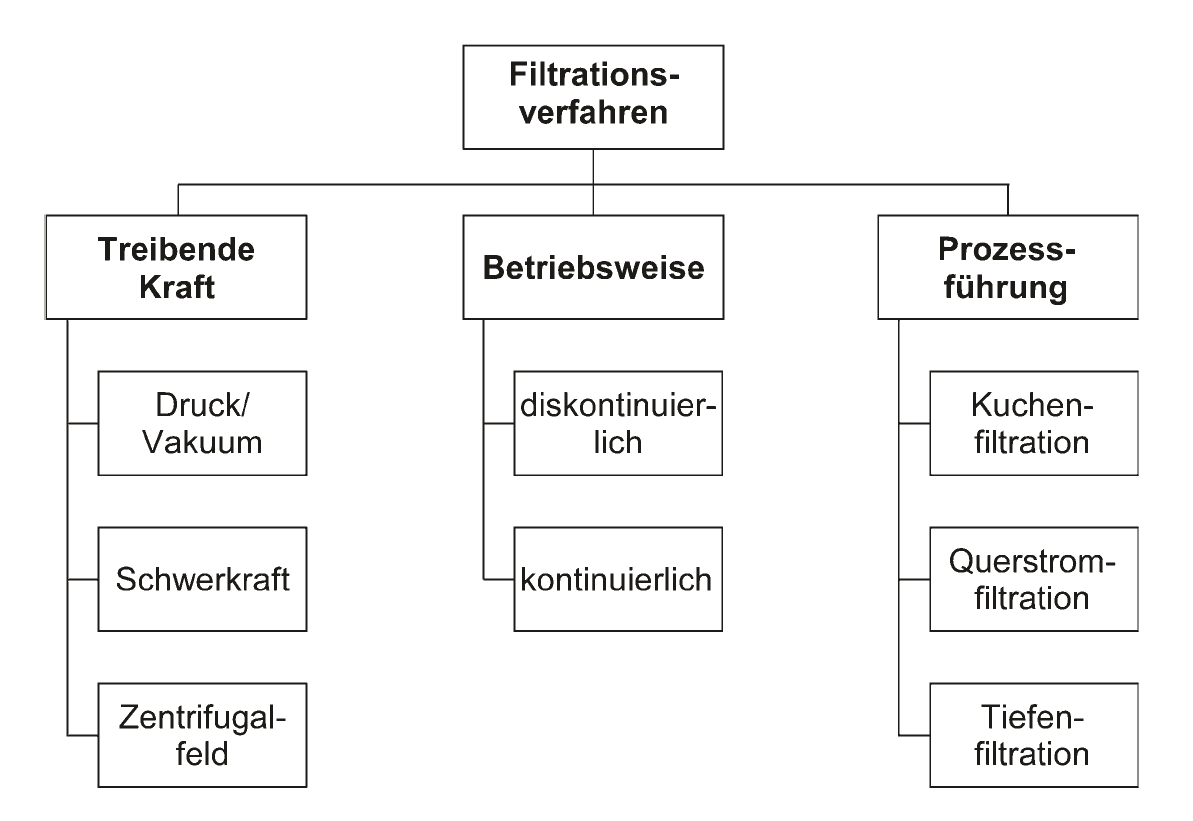
\includegraphics[width=0.8\linewidth]{images/klassifikation_filtrationsverfahren.png}
        \caption[Klassifikation Filtrationsprozesse]{Klassifikation der Filtrationsverfahren nach Kraume \cite{transportvorgänge} }
        \label{fi:klassifikation_filtration}
    \end{center}
\end{figure}
\subsection{Filterparameter}
Da die Abstände einzelner Filterfasern um ein vielfaches größer als die Partikeldurchmesser sind, liegt der modellhaften Beschreibung in der Regel eine einzelne Filterfaser zugrunde.
Wichtigste Kenngröße für die Wirksamkeit eines Filters ist der \ac{eta}.  Dieser wird definiert als das Verhältnis der \ac{con} oder \ac{conM} des zu trennenden Stoffes an der Rohgasseite $c_0$ und der Reingasseite $c_1$.\cite{Staubabscheidung}
\[
\ac{eta} = \frac{c_0 - c_1}{c_0}
\]
In Bezug auf typische Angaben bei der Definition von Partikeln in Medien wäre hier die Verwendung der Mengenkonzentration zu erwarten, es wird jedoch in der Regel die Massenkonzentration verwendet. Mit Hinzunahme der Staubspeicherfähigkeit, welche die Fähigkeit des Filters beschreibt eine bestimmte Masse an Staub zu speichern, ensteht somit eine Grundlage für die Berechnung der Standzeit von Filtern bei der Auslegung der Anlage.
Die Staubspeicherfähigkeit ist hierbei abhängig von der Art des Staubes und einer vorgegebenen Druckdifferenz $\Delta p$, bis zu der der Wert für die Staubmasse gilt, und wird allgemein in Gramm angegeben. \cite{vdi3677_2} \newline
Während der Abscheidegrad \ac{eta} nur eine Aussage über die gesamte abgeschiedene Staubmenge ist, liefert der \ac{etaX} den Abscheidegrad von bestimmten Stäuben. \ensuremath{\bar x} ist hierbei der mittlere Teilchendurchmesser einer bestimmten Staubfraktion. Die Berechnung erfolgt analog zu \ac{eta}. \cite{immission} Unterschiedliche Abscheideprozesse und Filterelemente haben auch unterschiedliche Fraktionsabscheidegrade, und werden entsprechend je nach Anwendungsfall eingesetzt (s. Abb. \ref{fi:frak_filter}).
\begin{figure}[H]
    \begin{center}
        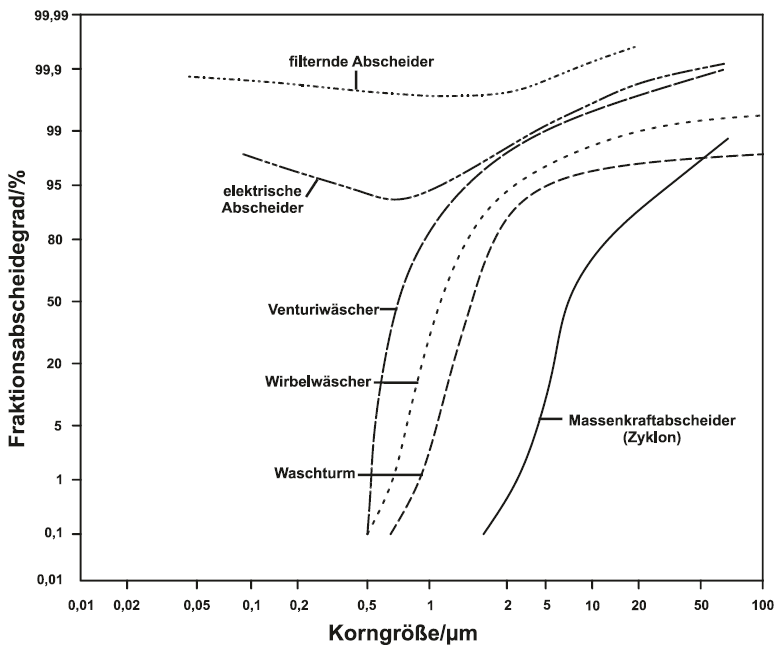
\includegraphics[width=\linewidth]{images/frak_filter.png}
        \caption[Fraktionsabscheidegrad verschiedener Abscheidesysteme]{Fraktionsabscheidegrad verschiedener Abscheidesysteme \cite{frak_filter} }
        \label{fi:frak_filter}
    \end{center}
\end{figure}
\subsection{Überblick über Filterbauarten}
\label{sec:filterbauarten}
Folgend soll ein Überblick über die unterschiedlichen mechanischen Filterbauarten geschaffen werden. Hierbei wird zuerst nur grob zwischen prinzipiellen Bauarten unterschieden, während folgend näher auf die für die Arbeit relevanten Filterbauarten zur Gebäudeklimatisierung und -belüftung eingegangen wird.
\newline
Massenkraftabscheider (Zyklone s. Abb. \ref{fi:zyklon}) zeichnen sich durch einen einfachen Aufbau und geringe Kosten aus. Sie sind besonders für die Abscheidung von Partikeln mit relativ großem mittleren Durchmesser (Grobstäube) geeignet, weswegen ihr Haupteinsatzgebiet die Vorentstaubung von Gasen ist (s. Verlauf \ref{fi:frak_filter}). Bei diesem Wirkpinzip wird die einströmende Luft in eine Kreisbewegung gezwungen, wodurch sich die Staubpartikel in Folge der Zentrifuglkraft an der Zyklonwand niederschlagen. Das Prinzip wird auch bei der Abreinigung von Flüssigkeiten eingesetzt, und wird auf Grund der hohen Betriebssicherheit und geringen Kosten in vielen Industriezweigen eingesetzt.\cite{immission} \newline
Nassabscheider, wie der Venturiwäscher (s. Abb. \ref{fi:venturi}), werden eingesetzt um staub- und gasförmige Schadstoffe abzuscheiden. Wegen der vergleichsweise hohen Betriebskosten werden sie vornehmlich bei kleinen Volumenströmen eingesetzt. Dies ist bedingt durch die Verlagerung des Schadstoffes vom Gas in die genutzte Flüssigkeit (meist Wasser), was eine aufwendige Nachbehandlung erforderlich macht. Entscheidend für die Abscheideleistung ist die Maximierung der Grenzfläche zwischen Tröpfchen und Gas, sowie die Relativgeschwindigkeit der Phasen zueinander. Der Venturiwäscher zählt deshalb zu den sog. Hochleistungswäschern, weil durch die hohen Relativgeschwindigkeiten eine gute Abscheideleistung erreicht wird. Nassabscheider haben jedoch den gemeinsamen Nachteil, dass ein hoher Druckwiderstand an Düse oder Diffusor entsteht, um eine gute Zerstäubung der Waschflüssigkeit zu erreichen. Das heißt, um eine effektive Reinigung zu gewährleisten, muss die Fördereinrichtung für Gas bzw. Flüssigkeit eine entsprechende Leistung erbringen. \cite{immission} \newline
Elektroabscheider (s. Abb. \ref{fi:elektroabscheider}) werden zur Abreinigung großer Volumenströme bei höheren Temperaturen, z.B. in Kraftwerken und Hütten eingesetzt. Die Schadstoffpartikel werden dabei elektrisch aufgeladen, und an einer Niederschlagselektrode abgeschieden. \cite{immission} Über eine Gleichspannung von 30-100 kV werden Elektronen von einer Sprühelektrode aus stark beschleunigt. In Folge werden Gasmoleküle ionisiert, welche wiederum die Staubpartikel negativ aufladen und an die Abscheidewand bzw. Niederschlagselektrode mitreissen. \cite{immission}Hierdurch bildet sich eine Staubschicht an der Niederschlagselektrode, welche als Isolator wirkt, und deshalb periodisch wieder abgetragen werden muss. \newline
Filter besitzen von allen Abscheideverfahren fast unabhängig vom Korndurchmesser die höchsten Abscheidegrade. Nachteil ist, insbesondere bei Tiefenfiltern, die geringe Speicherkapazität, was ihre Einsatzmöglichkeiten einschränkt. Bezeichnend ist die Vielzahl unterschiedlicher Bauformen und Filterwerkstoffe (s. Abb. \ref{fi:filterelemente}). Sie werden allgemein zwischen Oberflächen- und Tiefenfiltern unterschieden (s. Abb. \ref{fi:tiefen_oberfläch}). Bei Oberflächenfiltern bildet sich an der Rohgasseite ein Filterkuchen, welcher selbst als Filter wirkt. Die Zusetzung beider Filtergruppen hat einen zunehmenden Druckverlust am Filter zur Folge, und ist eine wichtige und betriebsrelevante Größe (s. Abb. \ref{fi:druckverlust_abr}). Der Filterkuchen wird periodisch wieder abgetragen. Hierbei werden Vibrationen/Rütteln, oder auch Druckimpulse/Pneumatik eingesetzt. Häufigstes Verfahren hierfür ist ein Gegenspülen im Online-Betrieb mittels Klappensteuerungen in den Rohrelementen.\cite{Staubabscheidung} Ziel ist die Regeneration des Filters, allerdings tritt immer eine gewisse Tiefenfiltration, und folglich Verschleiß auf, wodurch die Filterelemente getauscht werden müssen. Filter gehören zu den ältesten Abscheideverfahren, ihrer geringen chemischen- und Temperaturbeständigkeit konnte mit modernen Werkstoffen entgegengewirkt werden, wobei heute Glas- und Mineralfasern sowie diverse Kunstfasern wie Aramid bis Stahlfasern eingesetzt werden. Die Abbildung \ref{fi:filterelemente} verdeutlicht hierbei die Vielseitigkeit der unterschiedlichen Filterbauarten, deren häufigste Vertreter Schlauch- und Taschenfilter sind. \cite{immission}
\begin{figure}[ht!]
    \begin{center}
%
       \subfigure[Zyklon]{%
           \label{fi:zyklon}
           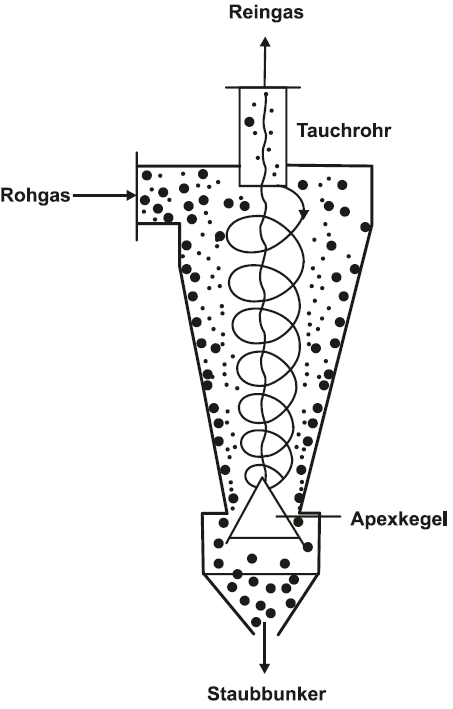
\includegraphics[width=0.5\textwidth]{images/zyklon.png}
       }%
       \subfigure[Venturiwäscher]{%
          \label{fi:venturi}
          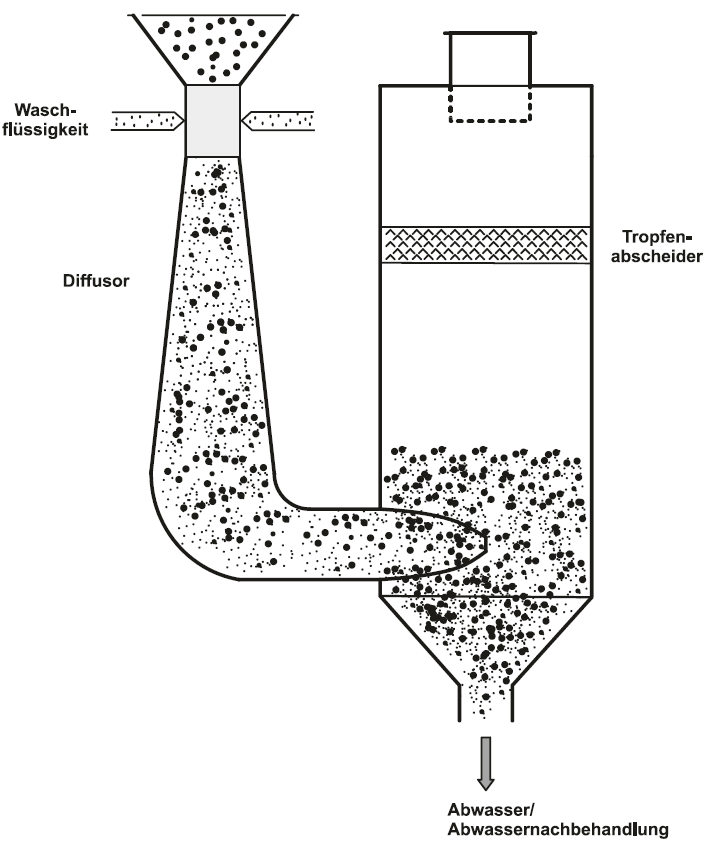
\includegraphics[width=0.5\textwidth]{images/venturi.png}
       }\\ %  ------- End of the first row ----------------------%
       \subfigure[Elektroabscheider]{%
           \label{fi:elektroabscheider}
           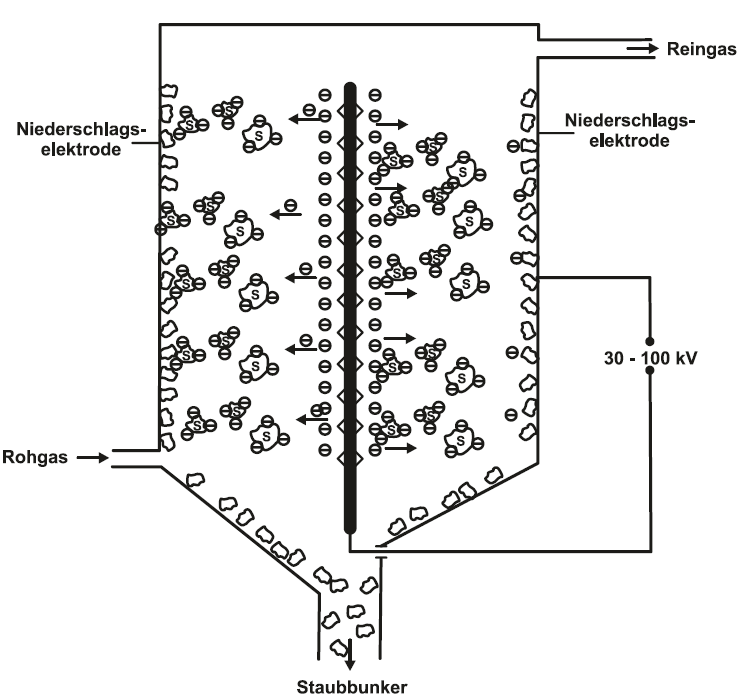
\includegraphics[width=0.5\textwidth]{images/elektro.png}
       }%
       \subfigure[Filterelemente]{%
           \label{fi:filterelemente}
           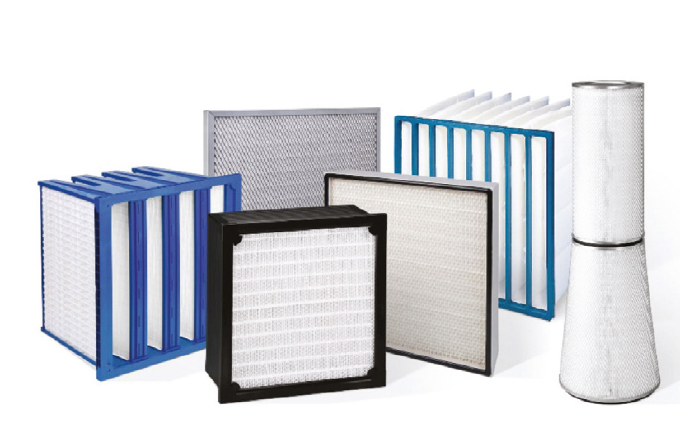
\includegraphics[width=0.5\textwidth]{images/filterelemente.png}
       }\\%
%
   \end{center}
   \caption{%
       Unterschiedliche Verfahrensprinzipien zur Staub- und Aerosolabscheidung; Quellen: \ref{fi:zyklon} - \cite{zyklon}; \ref{fi:venturi} - \cite{venturi}; \ref{fi:elektroabscheider} - \cite{immission}; \ref{fi:filterelemente} - \cite{filterelemente}
    }%
  \label{fig:verfahren}
\end{figure}
\newpage
\subsection{Filtereffekte}
\label{sec:filtereffekte}
Bei der Abscheidung von Partikeln aus Medien wirken unterschiedliche Filtereffekte. Diese Effekte treten je nach Größe (Durchmesser) der Partikel und Filterart unterschiedlich stark auf. Folgend werden diese Effekte kurz dargestellt, wobei die Effekte absteigend mit Hinblick auf die Stärke des Effekts bei kleiner werdender Partikelgröße geordnet sind. Bei einer detaillierten Untersuchung mit variiertem Volumenstrom können sich die Anteile der wirkenden Effekte deutlich verschieben, was signifikanten Einfluss auf die Filterleistung hat.
\begin{figure}[H]
    \begin{center}
        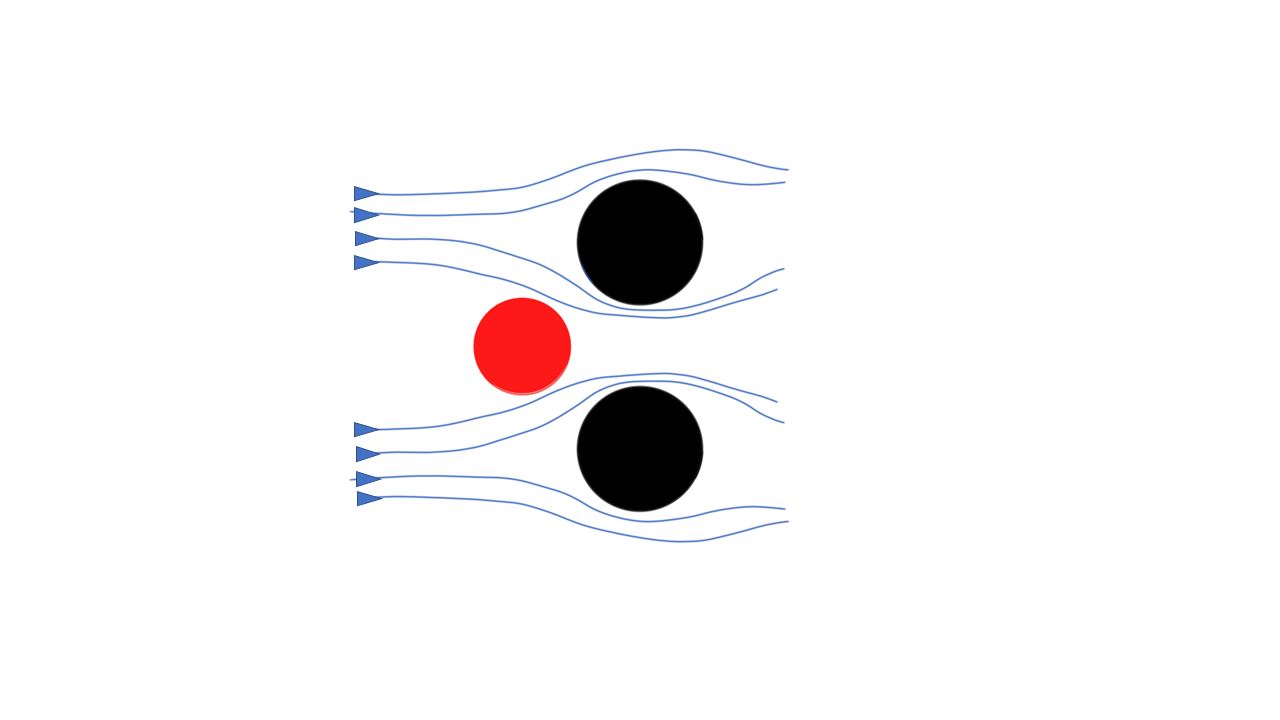
\includegraphics[width=\linewidth]{images/sieb2.png}
        \caption[Siebwirkung]{Prinzipskizze Siebwirkung}
        \label{fi:siebwirkung}
    \end{center}
\end{figure}
Wenn der Durchmesser der Partikel größer ist als der Abstand der Filterfasern zueinander, kann der Partikel das Filtermaterial nicht durchdringen. (siehe Abb. \ref{fi:siebwirkung}) Folglich tritt der Effekt verstärkt mit zunehmender Strömungsgeschwindigkeit und Größe bzw. Masse der Partikel auf. Der Siebeffekt ist im Fall von Tiefenfiltern bei der Beurteilung der Abscheidung quasi irrelevant, denn die Porosität der genutzten Filtermedien liegt bei bis zu 99,8 \% , folglich liegen die Fasern um ein vielfaches weiter auseinander, als der Durchmesser der abgeschiedenen Partikel. \cite{vdi3677_2} Bei Oberflächenfiltern wird der Siebeffekt, zumindest in der VDI Richtlinie 3677 - Blatt 1 "Filternde Abscheider - Oberflächenfilter" \cite{vdi3677_1}, nicht explizit als relevanter Effekt aufgeführt. 
\begin{figure}[ht!]
    \begin{center}
%
       \subfigure[Trägheitseffekt]{%
           \label{fi:traegheit}
           \includegraphics[width=0.5\textwidth]{images/trägheit.png}
       }%
       \subfigure[Sperreffekt]{%
          \label{fi:sperrefekt}
          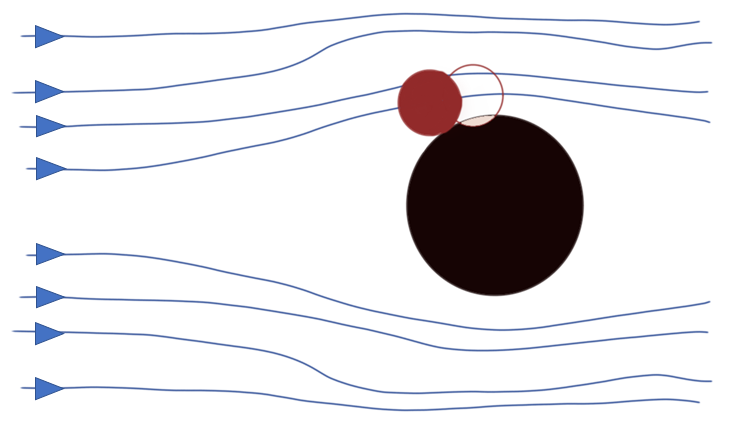
\includegraphics[width=0.5\textwidth]{images/sperr.png}
       }\\ %  ------- End of the first row ----------------------%
       \subfigure[Diffusionseffekt]{%
           \label{fi:diffusion}
           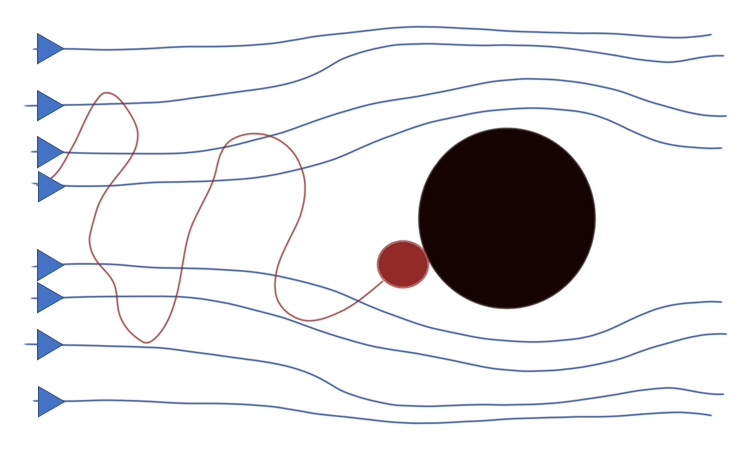
\includegraphics[width=0.5\textwidth]{images/diffusion2.png}
       }%
       \subfigure[Elektrostatische Anziehung]{%
           \label{fi:elektrostatisch}
           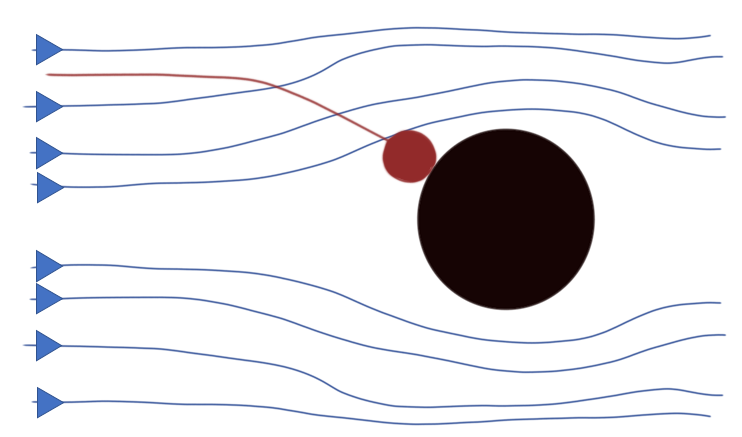
\includegraphics[width=0.5\textwidth]{images/elektrostatisch1.png}
       }\\%

%
   \end{center}
   \caption{%
       Prinzipskizzen von Filtereffekten, welche bei der Partikelabscheidung mit Faserfiltern auftreten
    }%
  \label{fig:filtereffekte}
\end{figure}
Relativ große, oder schwere, Partikel sind auf Grund ihrer Masse zu träge um dem Luftstrom um die Filterfaser zu folgen (siehe Abb. \ref{fi:traegheit}). Dadurch kommen sie mit der Faser in Berührung und bleiben dort hängen. 
Leichtere Partikel folgen hingegen der Strömung um die Faser. Genauer folgt der Masseschwerpunkt des Partikels der Strömung um die Faser. Wenn der Abstand dieses Punktes zur Faser den Abstand des Punktes zur Außenkontur des Partikels unterschreitet, bleibt der Partikel durch Adhäsionskräfte haften. Dieser Vorgang wird als Sperreffekt bezeichnet (siehe Abb. \ref{fi:sperrefekt}). Hierbei begünstigen große Partikeldurchmesser im Verhältnis zum Faserdurchmesser die Wahrscheinlichkeit eines Auftreffens auf die Faser. Der Effekt wird mathematisch mit dem \ac{R} in Abhängigkeit der \ac{d} von Faser~$\ac{d}_{F}$ und Partikel~$\ac{d}_{P}$ beschrieben. \cite{vdi3677_2} 
\[
R = \frac{d_P}{d_F}
\]

Der Sperreffekt ist insbesondere bei Oberflächenfiltern mit Filterkuchen der primäre Abscheidemechanismus. \cite{vdi3677_2} 
Bei kleinen Durchmessern ( \ac{d} kleiner 1 \si{\micro\metre} \cite{Grundlagen_Filtertechnik} bzw. kleiner 0,5 \si{\micro\metre} \cite{vdi3677_2} )folgen die Partikel nicht mehr allein der Strömung. Geringe \ac{u} von \ac{u} $<$ 0,1 \si{\metre\per\second} begünstigen ebenfalls den sog. Diffusionseffekt (s. Abb. \ref{fi:diffusion}).
Es treten auch Transportmechanismen durch elektrostatische Kräfte zwischen Partikeln und Filtermedium auf (s. Abb. \ref{fi:elektrostatisch}). Diese treten auf, wenn Partikel bzw. Filtermedium elektrostatisch aufgelagen sind, was in manchen Filtern gezielt herbeigeführt wird \cite{vdi3677_2}. Die Abschätzung des Einflusses, und das Design solcher Filter ist eher speziell, und basiert auf Approximationsgleichungen (s. auch \cite{faser_elektro}).
\subsection{Filterklassen Luftfilter}
\label{sec:filterklassen}
Um schädliche Effekte auf Umwelt und Menschen abzuwenden, müssen Filter in der Lage sein unterschiedliche Aerosole herauszufiltern. Diese Aerosole können z.B. in der Luft schwebende Metallfragmente, Faserreste, sowie Organsimen wie Pilzsporen, Pollen und Keime sein. Für die Gesundheit ist neben dem Schadstoffgehalt bzw. Toxizität der Partikel die Größe der Staubpartikel der entscheidende Parameter. \cite{Grundlagen_Filtertechnik} Partikel mit einem Durchmesser größer als 10 µm werden als Grobstaub bezeichnet. Dieser Grobstaub bleibt in den Härchen und Schleimhäuten des Nasen-Rachenraums hängen. Kleinere und kleinste Staubpartikel, sog. Feinstaub können diese natürlichen Filter durchdringen, und werden daher als inhalierbar bzw. alveolengängig bezeichnet. \newline
Basierend auf dieser Unterscheidung werden ebenso die eingesetzten Filterklassen zwischen Grobstaubfilter und Feinstaubfilter unterschieden. Bei noch kleineren zu filternden Partikelgrößen, beispielsweise bei Reinraumanwendungen kommen sog. Schwebstofffilter zum Einsatz. Diese unterscheiden sich jedoch in Hinblick auf die Anteile der wirkenden Filtereffekte von den anderen beiden beschriebenen Filterarten. \newline
Staubfilterklassen werden eigentlich seit Mitte 2018 nicht mehr nach EN 779 klassifiziert (s. Abb. \ref{fi:filter_gmf}), die veralteten Klassen finden aber noch Verwendung in Asien, und werden auch immernoch in z.B. Produktkatalogen von Filterherstellern angegeben. Auf die Prüfverfahren soll hier nicht im Detail eingegangen werden, es ist für das Verständnis der Arbeit jedoch wichtig zu bedenken, das auch der sog. synthetische Staub (ASHRAE-Staub), wie auch der Staub mit durchschnittlichen Partikeldurchmessern von 0,4 µm, selbst genormt ist (Prüfstaub). Im Rahmen der Vergleichbarkeit unterschiedlicher Filter ist dies unvermeidbar, entsprechend kann eine Prüfung aber niemals die Realität abbilden, da die Staubzusammensetzung ein variabler Eingangswert ist. Die Geltungsbereiche der Abscheidegrade sind außerdem nur bis zu einer definierten Enddruckdifferenz garantiert bzw. geprüft. Die Mindesteffizienz bezeichnet den mindestens erreichten Abscheidegrad des schlechtesten Prüfergebnisses eines Filters aus einer Prüfreihe. Grobstaubfilter werden bei der Prüfung nicht mit 0,4 µm Staub beaufschlagt.\cite{Grundlagen_Filtertechnik}
\begin{figure}[H]
    \begin{center}
        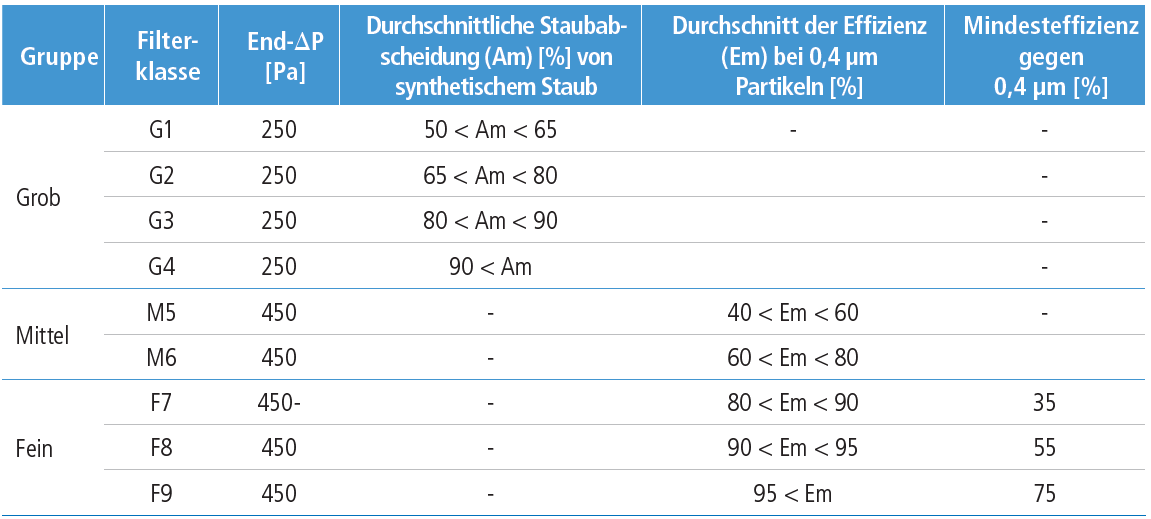
\includegraphics[width=\linewidth]{images/filter_GMF.png}
        \caption[Filterklassen]{Filterklassen Grob, Mittel, Fein nach EN 779}
        \label{fi:filter_gmf}
    \end{center}
\end{figure}
Mit neuen Erkennnissen über die Schädlichkeit von Feinstaub für die Gesundheit wurde eine Neuerung der Normen zur Klassifizierung von Filtern angestoßen. Diese Entwicklungen mündeten in einer neuen Norm ISO 16890 \cite{16890}. Da die reale Verteilung der Partikelgrößen nicht den festen 0,4 µm nach EN 779 entspricht, ist diese Prüfung realitätsnäher. Die neue Gruppierung ePMx beschreibt dabei die gesamte Staubfraktion von 0,3 µm bis x µm (s. Abb. \ref{fi:epmX}). Coarse beschreibt hierbei Filter, die für Partikelgrößen von 0,3 - 10 µm einen Abscheidegrad von 50 \% unterschreiten. Zusätzlich wird eine Angabe über den Durchschnitt zwischen Anfangs- und Mindest-Abscheidegrad bei der Prüfung gemacht, wobei  auf 5\%-Schritte gerundet wird. Beispielsweise beschreibt ein Filter ISO ePM10 85\% einen Filter, der im Bereich PM10 (0,3 - 10 µm) einen Abscheidegrad von 85 - 90\% erreicht.
\begin{figure}[H]
    \begin{center}
        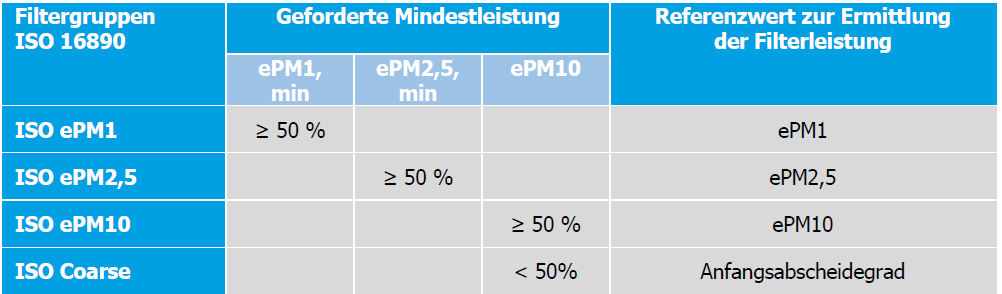
\includegraphics[width=\linewidth]{images/epmX.png}
        \caption[Filtergruppen ISO 16890]{Einteilung der Filtergruppen nach ISO 16890 \cite{altneu}, \cite{16890}}
        \label{fi:epmX}
    \end{center}
\end{figure}
Für Stäube im Sub-µm Bereich werden Schwebstofffilter eingesetzt. Diese Filter liefern die höchsten Abscheidegrade der mechanischen Luftfiltration, und werden primär als finale Filterstufe bei hochsensiblen Prozessen, wie OP-Räumen, Reinräumen und militärischen Anwendungen eingesetzt. Desweiteren werden Schwebstofffilter zur sicherheitsrelevanten Abluftbehandlung, z.B. bei der Asbestsanierung oder Nuklearindustrie, eingesetzt. \newline 
Schwebstofffilter sind dabei in der Lage extrem kleine Partikelgrößen, wie Viren, Bakterien und nanoskopische Stäube abzuscheiden. Relevante Normen sind hierbei EN 1822 \cite{1822} und ISO 29463, sie sind daher entkoppelt von der Neuerung bei den anderen Staubfiltern.
Die Qualitätsansprüche an Prüfung, Produktion und Installation solcher Filter sind entsprechend hoch. Hierfür wird zunächst mit dispersen Prüfaerosolen die \ac{MPPS} bestimmt, und der Filter anschließend anhand dieser geprüft. Während bei \ac{epa}-Filtern nur Abscheide- und Durchlassgrad des gesamten Filters geprüft werden, erfolgt bei \ac{hepa} und \ac{ulpa} Filtern zusätzlich eine Prüfung auf Leckagen. Die Filtermedien sind meist empfindlich gegenüber mechanischen Belastungen. \cite{Grundlagen_Filtertechnik} Bei der Produktion auftretende Toleranzschwankungen und kleinste Verklebefehler führen zu lokal stark erhöhten Partikeldurchlässen. Bei diesem Prüfschritt wird mit Prüfnebel und optischen Verfahren zunächst die schwächste Stelle(n) des Filters ermittelt, und diese anschließend gezielt mit dem \ac{MPPS}-Staub geprüft (Gruppierungen s. Abb. \ref{fi:filter_ehu}).
\begin{figure}[H]
    \begin{center}
        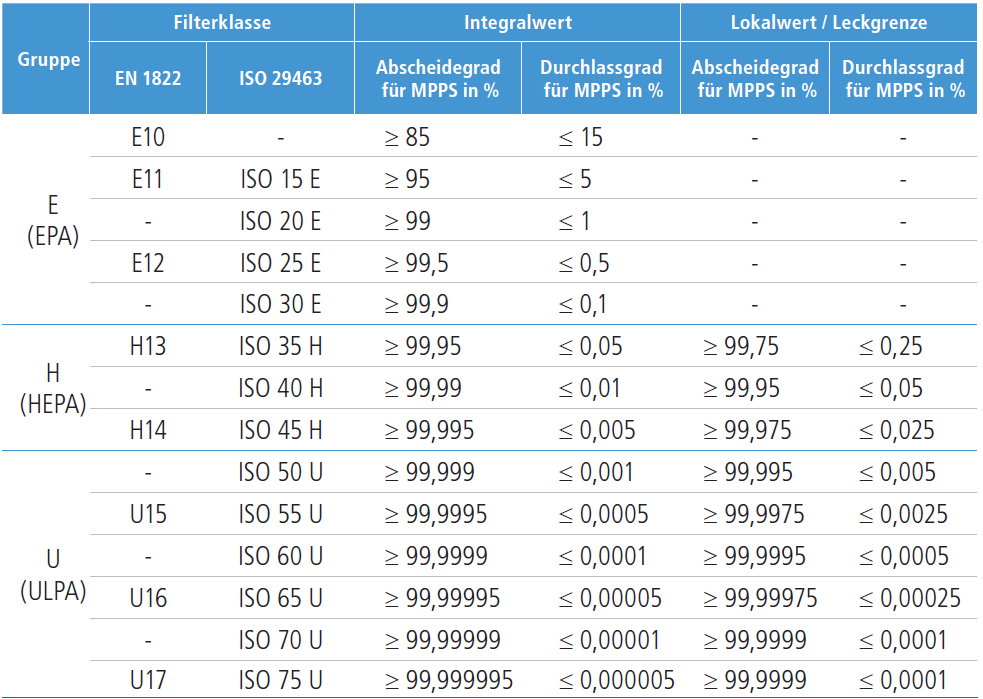
\includegraphics[width=\linewidth]{images/filter_EHU.png}
        \caption[Filterklassen Schwebstoffe]{Schwebstofffilterklassen EPA, HEPA, ULPA nach DIN EN 1822 \cite{1822}}
        \label{fi:filter_ehu}
    \end{center}
\end{figure}
\subsection{Aufbau von Raumlufttechnischen Anlagen}
\label{sec:aufbau}
Der Aufbau von Raumlufttechnischen Anlagen ist so vielfältig wie die Einsatzzwecke der ausgerüsteten Gebäude. Eine Vorstellung sämtlicher zu berücksichtigenden Eigenschaften bei der Planung solcher Anlagen würde zu viel Raum in dieser Arbeit fordern. Stattdessen wird folgend auf die für die Arbeit relevanten Aspekte solcher Anlagen eingegangen. \newline
Grundlegendes Entscheidungsmerkmal von Raumlufttechnischen Anlagen nach Bohne \cite{tavg} ist die Unterscheidung zwischen Anlagen mit Lüftungsfunktion und solchen ohne Lüftungsfunktion. Im Rahmen dieser Arbeit ist eine Lüftungsfunktion Vorraussetzung für die Sinnhaftigkeit einer Filterüberwachung.
Anlagen können zusätzlich, unabhängig von der Lüftungsfunktion, folgende Aufgaben erfüllen:
\begin{itemize}
    \item H - Heizen
    \item K - Kühlen
    \item B - Befeuchten
    \item E - Entfeuchten
\end{itemize}
Eine Anlage, die nur Luft transportiert (und ggf. filtert), wird Lüftungsanlage genannt. Wird keine Außenluft zugeführt handelt es sich um eine Umluftanlage. Diese Definition umfasst ebenfalls Anlagen, die maximal eine der genannten Behandlungsfunktionen erfüllen. Werden zwei oder drei Teilfunktionen erfüllt wird die Anlage als Teilklimaanlage, respektive Umluftteilklimaanlage bezeichnet.
Nur wenn alle Teilfunktionen erfüllt werden handelt es sich um eine (Umluft-)Klimaanlage. \newline
Weitere Unterscheidungen erfolgen dann auf Grundlage des genutzten Mediums zum Temperaturmanagement bswp. Wasser, Kühlmittel.\cite{tavg}
Im Kontext der Fragestellung hochinterssant ist die Grundkategorie der Regelung oder Steuerung (s. Abb. \ref{fi:regelungsarten}), sowie die hierbei auftretender Besonderheiten, die einen denkbaren Einfluss auf den Filterverschleiß haben können.
\begin{figure}[H]
    \begin{center}
        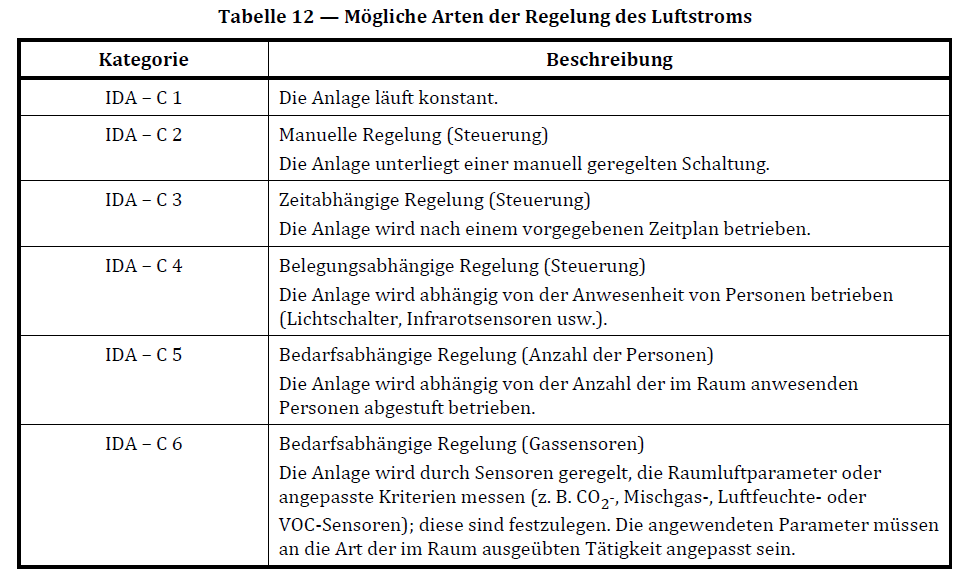
\includegraphics[width=\linewidth]{images/arten_regelung.png}
        \caption[Regelungsarten Luftstrom]{Grundkategorien Regelung aus DIN EN 16798-3 \cite{16798} }
        \label{fi:regelungsarten}
    \end{center}
\end{figure}
Es ist ebenfalls relevant, ob die Regelung für einzelne Räume oder zentralisiert für Gebäudebereiche realisiert wird. Unabhängig hiervon ist für die Belastung der Filter der Volumenstrom von zentraler Bedeutung. Bei den Klassen IDA-C4 und niedriger wird ein fester Sollwert für den Volumenstrom bei der Auslegung festgelegt. Das heißt im Sinne einer Überwachung des Filerverschleißen ist hier prinzipiell nur die Betriebsdauer zu erfassen. Bei den Klassen IDA-C5 und C6 wird dieser Sollwert jedoch bedarfsorientiert angepasst, und muss somit als zusätzliche zeitvariante Variable in das Modell zur Vorhersage einfließen. Die Norm weißt in diesem Fall auf Druckschwankungen hin, welche durch den variierbaren Luftvolumenstrom verursacht werden können. \cite{16798} Diese müssten im Rahmen von Messungen unter Betriebsbedingungen erfasst werden, da sie von den örtlichen Gegebenheiten wie z.B. Windstärke und Anlagenmerkmalen abhängig sind. \newline
Bei Grobstaubfiltern ist in der Regel außerdem der Nennvolumenstrom bzw. Anströmgeschwindikeit einzuhalten, während bei Feinstaub- und Schwebstofffiltern je nach Bauform Abweichungen von +20\% bis -90\% zulässig sind.\cite{Grundlagen_Filtertechnik} Dies ist durch die wirkenden Filtereffekte bei Grobstaubfiltern bedingt, die stark von der Strömungsgeschwindigkeit abhängig sind (s. Kap. \ref{sec:filtereffekte}).
Der Fokus dieser Arbeit liegt auf dem Konzept bzw. der Machbarkeit. In diesem Rahmen wird der Volumenstrom als belegungsgesteuert angenommen, Einzelheiten der Anlagengestaltung vereinfacht, und eine Volumenstromregelung zur Verhinderung von Druckschwankungen im System vorausgesetzt. Weitere Anforderungen an eine solche Anlage zur Realisierung einer prädiktiven Überwachung ergeben sich aus den folgenden Unterkapiteln, und umfassen Möglichkeiten zur digitalen Datenerfassung, Netzwerkfähigkeit (Nutzung von Bussystemen), sowie Rechenkapazitäten.
\section{Grundlagen IIoT}\label{sec:iiot}
Das \ac{iiot} ist die Adaption des \ac{iot} auf die industrielle Produktionslandschaft. Die Grenzen zwischen den Begriffen \ac{cps}, \ac{iot} und \ac{i40} sind dabei fließend, und somit sinnbildlich für den neuartigen und volatilen Charakter der hintergründigen Technologien.
Grundsätzlich werden hierbei zahlreiche physikalische Objekte, sog. "Things", mit der Fähigkeit ausgestattet Informationen zu übertragen, und als Netzwerk (Internet) miteinander verknüpft. Dabei können die Things selber sowohl als Server als auch als Client agieren. Aufgaben wie z.B. Datenaggregation und -analyse können hierbei von den Things übernommen werden. Digitale Prozesse laufen also nicht mehr zwangsläufig  auf einem einzigen, monolithischen Server(cluster)-System ab, sondern zunehmend dezentralisiert.

"Grundidee [...] ist die Integration und
Vernetzung unterschiedlicher intelligenter Objekte in einem Produktionsumfeld. [...], dass mithilfe von Cloud Computing und analytischen
Auswerteverfahren, die wesentlichen Informationsbausteine
gewonnen werden können, die zu
effizienteren Serviceprozessen und zu einem optimierten
Kosten-Nutzenverhältnis führen. Für
Maschinen- und Anlagenbauer kommt heute die
Kombination von Produkt und Dienstleistung
im Sinne eines Product Service Systems immer
stärker in den Fokus." \cite{i40_instandhaltung}

Hierbei stellt die Integration eines Sensornetzwerkes in das Produktionsumfeld, mit dem Ziel einen Datenstrom zu erzeugen, die Grundlage. Ausgehend von diesem Datenstrom kann das Unternehmen kontinuierlich und in Echtzeit Informationen über seine physikalischen und virtuellen Bestandteile sammeln.
\ac{iiot} meint somit einen Bestandteil eines Szenarios, bei dem, innerhalb einer Cloud-Infrastruktur, z.B. automatisierte Funktionen zur Datenanalyse eingebunden werden. Hierdurch werden neue Nutzenpotenziale für das Unternehmen erschlossen. \cite{i40_instandhaltung}
Ein Beispiel hierfür wäre das Abrufen von Produktionsmessdaten vor der Bestellung durch den Kunden in einem Webshop. Der Kunde kann im Prusa Onlineshop für Filamente für \ac{fdm} 3D-Drucker während der Bestellung die Messdaten des Filamentdurchmessers, welcher einer der entscheidenden Faktoren für eine hohe Druckqualität ist, aus der Produktion abrufen (siehe Abb. \ref{fi:prusa}). Dies steigert das Kundenvertrauen in die Produktqualität, was wiederum einen erhöhten Umsatz für das Unternehmen generiert.
\begin{figure}[H]
    \begin{center}
        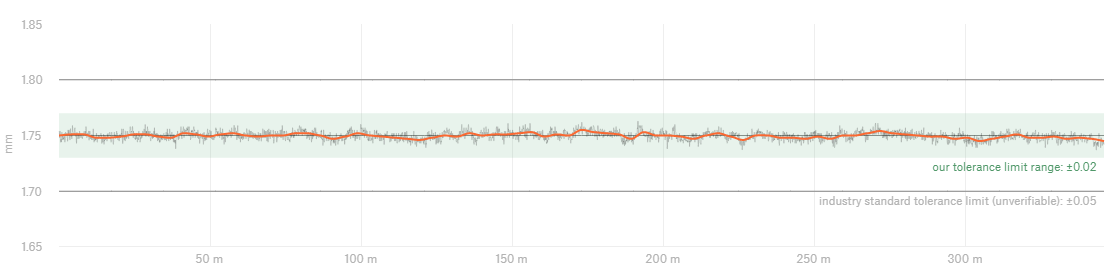
\includegraphics[width=\linewidth]{images/prusa.png}
        \caption[Prusament]{Prusa PLA Filament 1.75mm \cite*{prusa} }
        \label{fi:prusa}
    \end{center}
\end{figure}
Nicht zu unterschätzen ist hierbei in der Realität allerdings der Integrationsaufwand, welcher weit über den Aufbau eines Sensornetzwerkes mit eventueller Datenbank hinausgeht. Um ein solches System auch gewinnbringend einzusetzen ist es nötig \ac{api}'s für diverse Backendservices bereitzustellen. Desweiteren müssen diese Services auch anwendungsorientiert entwickelt bzw. programmiert werden, und schlussendlich auch in interne Systeme, wie z.B. \ac{erp} und \ac{bi} integriert zu werden.
Ein noch weiter gehender Schritt ist in diesem Zuge eine Schnittstelle zu den Systemen externer Dienstleister herzustellen, bspw. zur schnelleren Abwicklung von Wartungsaufträgen für Produktionsanlagen. Dies erfordert einheitliche Übertragungsstandards, und wird durch einander ähnliche Datenmodelle erleichtert.
\subsection{Architektur von IIoT Netzwerken}
Sollen die physischen Objekte im digitalen System lediglich repräsentiert werden, reicht eine Identifikation mittels \ac{qr} oder \ac{rfid} aus. Ein zentrales System kann nun die gekennzeichneten Objekte verfolgen und dem Nutzer relevante und aufbereitete Daten zur Verfügung stellen.
Sollen die Objekte selbst jedoch Daten verarbeiten, zum Beispiel ein Mikrocontroller der ein Sensorcluster ausliest und versorgt, benötigt dieser eigene Rechenkapazitäten, eine Datenschnittstelle bzw. Netzwerkanbindung und eine Energieversorgung, um Sensorwerte auszulesen, zu verarbeiten und für das System bereitstellen zu können. Diese Argumente machen deutlich, dass eine allgemeingültige Aussage zu der konkreten Architektur von \ac{iiot} Netzwerken nahezu unmöglich ist.
Derartige Netzwerke erfordern jedoch immer Übertragungsstandards, eine entsprechende Infrastruktur zur Datenübertragung, mehr oder weniger dezentralisierte Rechenkapazitäten, sowie Möglichkeiten zur Speicherung von Daten.
\begin{figure}[H]
    \begin{center}
        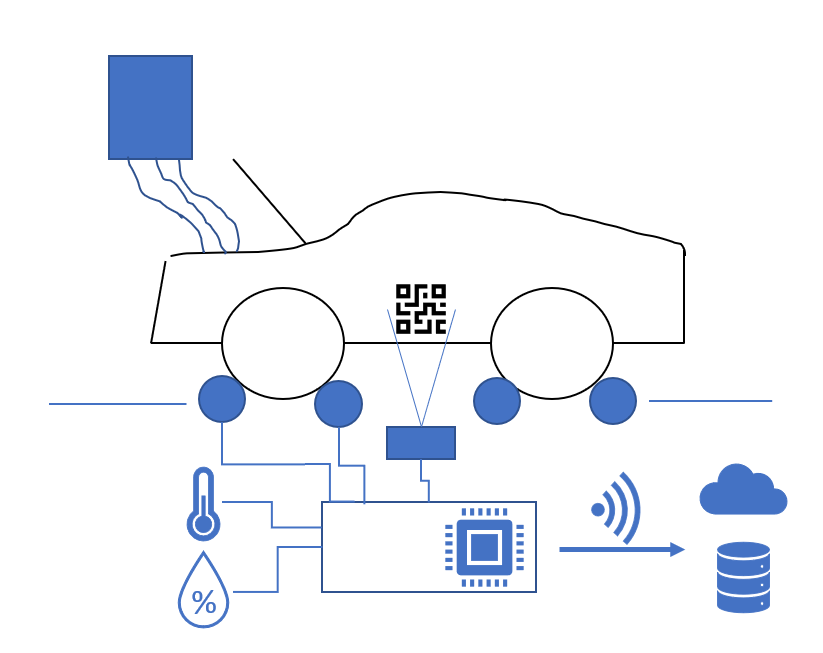
\includegraphics[width=\linewidth]{images/beispiel_iiot.png}
        \caption[Beispiel IIoT]{Auto Teststand mit IIoT Umsetzung}
        \label{fi:auto_iiot}
    \end{center}
\end{figure}
Der Teststand in Abbildung \ref{fi:auto_iiot}) soll heirzu als Beispiel dienen, und erfasst daher innerhalb eines eigenen Netzwerkes mit eigenen Protokollen und eigener Messdatenerfassung Umwelt-, Produkt-, und Testdaten. Die Zelle agiert dabei als autarkes \ac{cps}, und kann dabei Umwelteinflüsse auf Testparameter ausregeln. Ebenso ist es in der Lage die Testanalyse autonom von einem zentralen Server auszuführen, und z.B. Anomalien im Ablauf zu erkennen und zu melden. Die Testdaten werden drahtlos, in aggregierter und verknüpfter Form, an Backendservices für z.B. Produktivitätsdashboards gesendet. Während Rohdaten, wie Zeitreihen, über eine Cloud in spezialisierten Datenbanken hinterlegt werden. \newline Eine solche Architektur hat im Gegensatz zu einer traditionellen, monolithischen Architektur den Vorteil, dass der Datenstrom zu einem einzelnen Server(cluster) reduziert wird. Services für eine nachgelagerte Analyse, wie Prozessoptimierungen, können die Rohdaten je nach Bedarf von den Datenbanken abrufen. Die Testergebnisse müssen nicht von einem zentralen Server für mehrere Zellen parallel generiert werden, sondern werden direkt und aufbereitet an den Webserver für das Dashboard übergeben. Diese verzweigte Netzwerkarchitektur und Verteilung von Berechnungsaufgaben verringert den Netzwerktraffic, vermeidet Bottlenecks (Balancing von Serveranfragen) und berücksichtigt die Einschränkungen bei der Anzahl von Teilnehmern (z.B. Vergabe von IP-Adressen).
Hieraus ergibt sich jedoch der Nachteil des zusätzlich Wartungsaufwands, z.B. bei einem Variantenwechsel des Produkts. Moderne \ac{iot} Cloud Lösungen stellen hierfür Funktionalitäten bereit, um mehrere verknüpfte Things von einem einzigen, virtuellen Ort aus zu aktualisieren bzw. zu programmieren.
\subsection{Protokolle für Sensornetzwerke}
In Anlagen zur Klimatisierung, Belüftung, Heizung etc. von Gebäuden werden viele Sensoren und Stellglieder eingesetzt. Für eine echtzeitfähige Erfassung und Verarbeitung der Messgrößen, sowie Ansteuerung der Stellglieder reicht bei der üblichen Komplexität dieser Systeme eine analoge Datenübertragung über bspw. 5V- oder 10V-Technik nicht mehr aus. Digitale Transportmechanismen haben zudem den Vorteil geringerer Störanfälligkeit und die Fähigkeit Informationen über größere Strecken zu übermitteln. \cite{gebauto}
Um ein solches Kommunikationsnetzwerk bereitstellen zu können, sind sog. Bussysteme erforderlich. Diese ermöglichen eine Einbindung von Mess- und Regelgeräten in ein System. Beispiele hierfür sind Messumformer, Sensoren, Aktoren und Regler. \cite{61158-1} \newline
Auf Feldebene werden die üblichen analogen Datenübertragungen zwar durchaus noch genutzt, darüber hinaus hat die zunehmende Verfügbarkeit und die Verringerung der Kaufpreise von Mikrocontrollern in den 1980ern dazu geführt, dass Feldbus- und Bus-systeme in die \ac{glt} eingeführt wurden (s. Kap. \ref{sec:regelungsart}).
Die hierfür genutzten Protkolle sind über das ISO/OSI Schichtenmodell charakterisiert. Hierbei wird aufbauend auf die physikalische Schicht, welche die Übetragung von Informationen bitweise implementiert, mehrere Schichten mit abnehmenden Abstraktionsgrad der Informationen genutzt. Das hierfür weltweit verbreitete Referenzmodell beinhaltet sieben Schichten. \cite{osi} Diese setzen sich beispielhaft anhand eines Browserfensters wie folgt zusammen:
\begin{itemize}
    \item 7 - Application Layer      -   Browser Bedienelemente
    \item 6 - Presentation Layer     -   HTML-Rendering
    \item 5 - Session Layer          -  Tab-Browsing
    \item 4 - Transport Layer        -   TCP / UDP
    \item 3 - Network Layer          -   IP-Adressen
    \item 2 - Data Link Layer        -   MAC-Adressen
    \item 1 - Physical Layer         -   Digitale Signale
\end{itemize}
Die unterschiedlichen Schichten werden dabei von ebenso unterschiedlichen Hardware- bzw. Softwareschichten implementiert bzw. interpretiert.
Die in \ac{iiot} bzw. in der \ac{glt} genutzten Protokolle nutzen hierfür in der Regel die Schichten 1-4. Da die Daten lediglich in einem \ac{m2m} Szenario genutzt werden, und zudem Echtzeitfähigkeit zur Erfüllung von Regelungsaufgaben im Falle von \ac{ddc} Unterstationen gefordert wird, sind Session-Informationen i.d.R. überflüssig, bzw. führen zu einem inaktzeptablen Overhead.
\section{Grundlagen KI}
\label{sec:grundlagenKI}
Die Grundlagen für selbstlernende Algorithmen wurden bereits in den 50ern gelegt. Seitdem hat vorallem die immer stärker werdende Rechenleistung von Computern zu einem regelrechten Boom von \ac{ki} geführt. Es gibt mehrere Typen von \ac{ki}, wovon ein \ac{tnn} in Form eines Mehrschichtigen Feedforward-Netztes für den Anwendungsfall gut geeignet erscheint.\cite{ki} \newline
Sämtliche Ausprägungsformen und auch mathematische Einzelheiten vorzustellen soll an dieser Stelle nicht das Ziel sein. Vielmehr soll ein grundlegendes Verständnis für die genutzten Modell in \ac{KNIME} vermittelt werden. Eines der genutzten Modelle ist ein sog. Neuronales Netz.
Wie in Abb. \ref{fi:feedforward} zu sehen ist, breitet sich das Netz aus Perceptrons (vgl. Neuronen) von einem sog. Input Layer aus. Ein Perceptron ist in diesem Fall ein mathematisches Konstrukt, welches beliebig viele Eingaben gewichtet und miteinander verrechnet, und so ein Ergebnis erzeugt. In der einfachsten Form ist das Ergebnis 0, 1 oder -1; bei neueren Modellen oft auch von 0 bis 1. Der Input Layer repräsentiert hierbei einen Vektor, ferner einen Tensor, der die Eingangsparameter enthält. Ein beliebtes Beispiel ist die Bestimmung einer Blumenart anhand morphologischer Eigenschaften z.B. Blütendurchmesser, Länge Blütenstempel, Farbwert usw.. Die Zahlenwerte dieser Eigenschaften dienen nun als Eingaben für die nächste Schicht (Hidden Layer), deren Ausgaben (= 0...1) wieder mit jedem einzelnen Perceptron der nächsten Schicht verschaltet sind. Jede Linie in der Abbildung \ref{fi:feedforward} repräsentiert also einen Wert von 0 bis 1 und einen Gewichtungsfaktor.
Der Output Layer hat nun so viele Perceptrons wie die Anzahl an Klassen, die bestimmt werden sollen. Am Beispiel der Blumen also wie viele unterschiedliche Blumenarten bestimmt werden sollen. Die Output Perceptrons repräsentieren also jeweils eine Ergebnisklasse (vgl. Blumenart), und ihr Output, wiederum ein Wert zwischen 0 und 1, die Wahrscheinlichkeit, das es sich um die jeweilige Klasse (Blumenart) handelt.
\newline Entscheidend ist nun die Variation der Gewichtungsfaktoren der einzelnen Perceptrons durch ein Framework (Software), bis die errechnete Klassifikation mit einer ausreichenden Genauigkeit die Klassifikationen der Trainingsdaten abbildet. Hierfür werden viele Tausend Kombinationen an Gewichtungsfaktoren erzeugt, und die Ergebnisse verglichen. Moderne Frameworks können hierbei auch die Topologie des Netzes variieren. Ziel ist dann ein Netz, welches aus einem neuen Datensatz, anhand der erlernten Zusammenhänge, eine Entscheidung bezüglich der Ergebnisklasse errechnet. Dies offenbart auch einen Schwachpunkt solcher Netze, da nach Durchlaufen der ersten Schicht Informationen über die Dimension der Werte verloren gehen. Beispielsweise kann das Netz, auch bei einem Blütendurchmesser im km-Bereich, eine Klassifikation liefern, auch wenn eine solche Blume in der Realität nicht existiert. Man spricht daher im Kontext von KI auch von starker und schwacher Intelligenz, eine starke Intelligenz würde den offensichtlichen Fehler bzgl. des Blütendurchmessers registrieren, während eine schwache Intelligenz dies nicht kann.
\begin{figure}[H]
    \begin{center}
        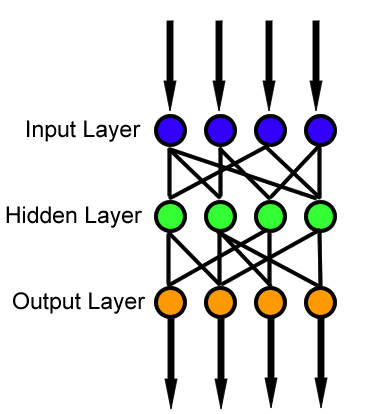
\includegraphics[width=0.7\linewidth]{images/feedforward.png}
        \caption[Feedforward Netz]{Informationsfluss Feedforward Netz \cite{feedforward}}
        \label{fi:feedforward}
    \end{center}
\end{figure}
\subsection{Decision Tree Learning}
\label{sec:dtl}
Entscheidungsbäume (engl. decision tree) werden bei Klassifikationsproblemen eingesetzt, um hierarchisch aufgebaute Entscheidungsregeln darzustellen. Bei jedem Knoten wird ein Attribut abgefragt, und somit der Datensatz immer weiter aufgeteilt, bis ein Blatt erreicht wird. Ein Blatt entspricht dabei der Klassifikation eines durch die vorherigen Knoten definierten Teils des Datensatzes in Bezug auf die Zielklasse. Im Beispiel \ref{fi:entscheidungsbaum} werden Apfelbäume anhand von Apfelbaum-typischen Attributen eingeteilt, um eine Aussage über das Ereignis \glqq Apfelbaum trägt Früchte\grqq{} (Zielklasse) zu treffen.\newline 
Das in \ac{KNIME} genutzte \ac{DTL} Modell basiert auf dem \ac{cart} Algorithmus. Allgemein wählt der \ac{cart} Algorithmus die Attribute zur Trennung der Daten nach der Maximierung des Informationsgehalts der resultierenden Datensätze aus. Hierbei werden Binärbäume generiert. Die Schwellenwerte für die numerischen Attribute an den Knoten, anhand deren die Trennung erfolgt, werden hierbei durch die Optimierung der Entropie der Subsets ermittelt, mit dem Ziel möglichst einheitliche Datensätze in Bezug zur Klasse zu erhalten. Entropie im Sinne der Informationstheorie meint hierbei ein Maß für die \glqq Reinheit\grqq{} bzw. den Informationsgehalt eines Datensatzes (s. Abb. \ref{fi:entropie}). Die Entropie ist dabei wie folgt definiert:
\[Entropie(p) = -\sum_{i=0}^n p_i {\log_2 p_i}\] 
Damit ergibt sich für die linke Menge in der Abbildung \ref{fi:entropie} mit $ p_1=\frac{7}{13}$ und $ p_2=\frac{6}{13}$ eine Entropie von $0,995$, während sich für die rechte Menge mit $ p_1=\frac{13}{13}$ und $ p_2=\frac{0}{13}$ eine Entropie von $0$ ergibt. Simpel ausgedrückt variiert also der Algorithmus die unterschiedlichen Trennungen im Verlauf des Baumes, bis möglichst eindeutige Datensätze in Bezug zur Zielklasse entstehen. Da die Klassifikation hierbei schlussendlich auf Vergleichsoperatoren beruht, ist dieser Algorithmus und auch der generierte Entscheidungsbaum in der Anwendung vergleichsweise schnell. In der Theorie kann der Baum immer weiter wachsen, bis er jeden Einzelfall des Trainingsdatensatzes absolut genau abdeckt. In der Praxis spricht man dabei vom sog. \glqq overfitting\grqq{}. In diesem Fall ist der Baum zu sehr spezialisert, und liefert somit kaum verallgemeinerbare Kenntnisse über die Klassifikation. Deswegen werden der Ausprägung des Entscheidungsbaums in der Praxis, wie auch in \ac{KNIME}, Grenzen gesetzt.
\begin{figure}[H]
    \begin{center}
        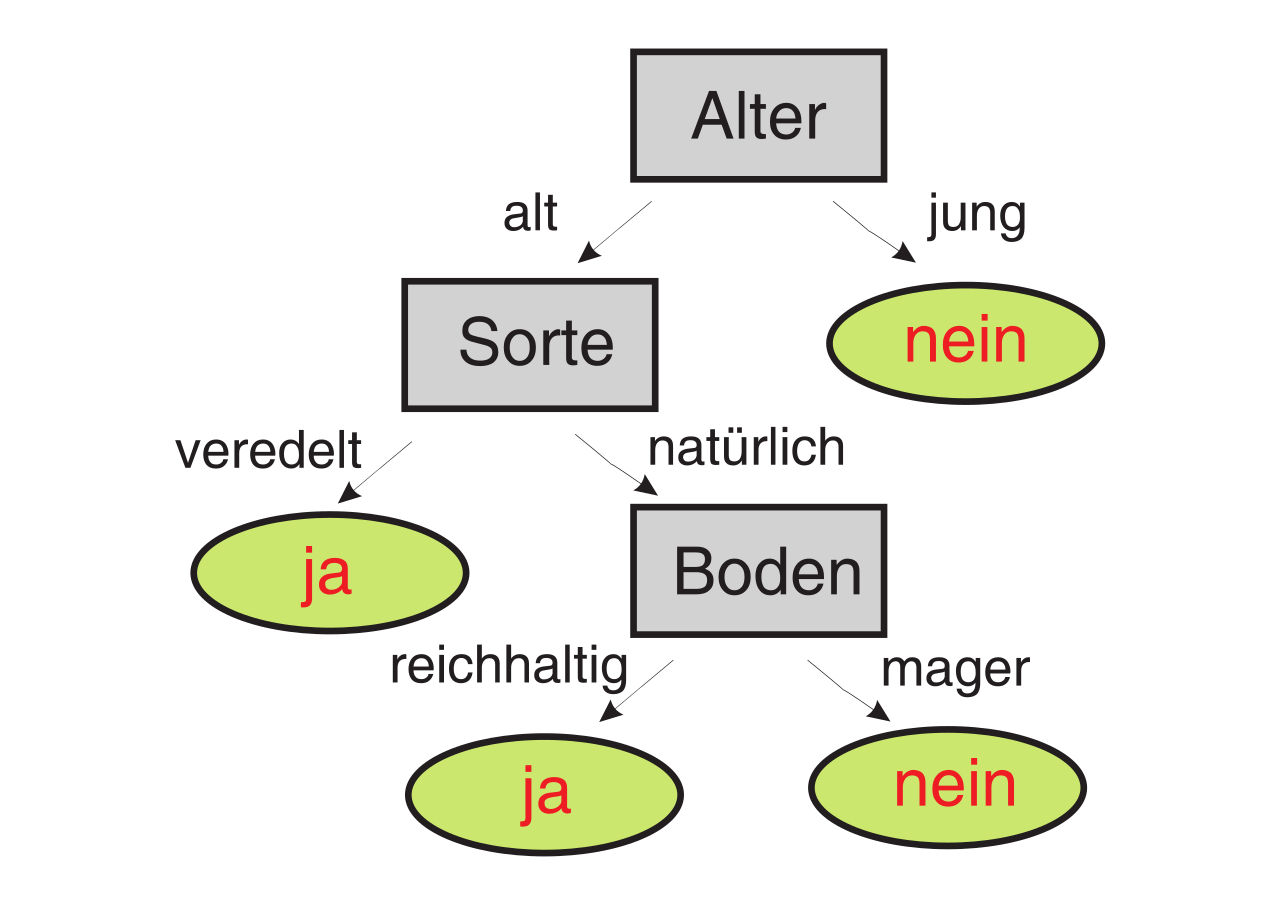
\includegraphics[width=\linewidth]{images/entscheidungsbaum.png}
        \caption[Binärer Entscheidungsbaum]{Binärer Entscheidungsbaum, ob ein Apfelbaum Früchte tragen wird \cite{entscheidungsbaum}}
        \label{fi:entscheidungsbaum}
    \end{center}
\end{figure}
\begin{figure}[H]
    \begin{center}
        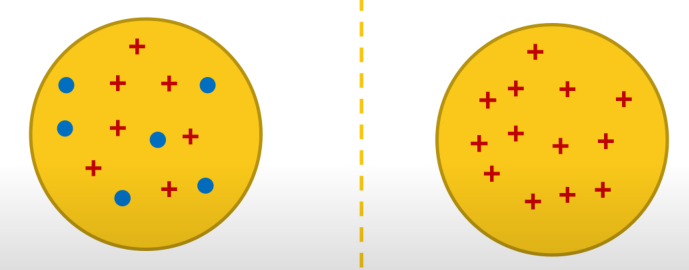
\includegraphics[width=\linewidth]{images/entropie.png}
        \caption[Darstellung Entropie]{Darstellung der Entropie zweier Datensätze mit hoher Entropie (links), und niedriger Entropie (rechts) \cite{entropie}}
        \label{fi:entropie}
    \end{center}
\end{figure}